   \item Wyrejestrowanie się klienta \\
 
 Opis słowny - jest to pierwszy przypadek użycia dla klienta, bez którego
 pozostałe przypadki nie mają racji bytu. Akcje w nim opisane mają miejsce, gdy
 użytkownik pierwszy raz pojawia się na stronie i po przejrzeniu oferty sklepu
 (co dostępne jest także dla użytkowników niezalogowanych) decyduje się na
 stworzenie konta i ewentualne rozpoczęcie zakupów. Obsługa tego przypadku
 użycia wymaga poprawnego procesowania operacji rejestracji i jej potwierdzenia.
 
 \begin{longtable}{|p{5cm}|p{7cm}|}
 	\hline
	\textbf{Aktor} & Klient \\
	\hline
	\textbf{Warunki początkowe} & Klient zalogowany, posiadający konto w systemi \\
	\hline
	\textbf{Opis przebiegu interakcji} & Podjęcie decyzji o wyrejestrowaniu,
	obsługa aktywnych zamówień
	\\
	\hline
	\textbf{Sytuacje wyjątkowe} & Brak\\
	\hline
	\textbf{Warunki końcowe} & Usunięcie klienta z systemu\\
	\hline
 \end{longtable}
 
  
  
  \item Wyrejestrowanie się klienta - scenariusz główny\\
  \begin{tabularx}{\linewidth}{ c X }
  Aktor: & Klient \\
  \end{tabularx}
  \begin{enumerate}
    \item Klient uruchamia witrynę internetową i loguje się na swoje konto
    (przypadek użycia Logowanie Do Systemu)
    \item Klient wybiera opcję usunięcia danych
    \item System sprawdza, czy istnieją niezrealizowane (oczekujące) zamówienia.
    Jeśli tak, wyświetla się alert z informacją, czy dane zamówienie zostało już
    wcześniej opłacone
    \item Jeśli istniały już zamówienia, które zostały opłacone a nie zostały
    jeszcze zrealizowane, system zleca odesłanie określonej kwoty pieniężnej z
    powrotem na konto użytkownika (z pominięciem kosztów obsługi)
    \item Klient zostaje poproszony o podanie przyczyn swojej decyzji -
    wypełnianie jest nieobowiązkowe
    \item Dane przechowywane są przez Okres Przechowywania Danych (wymaganie
    prawne - patrz Wymagania niefunkcjonalne punkt \ref{itm:OPD}). W tym
    czasie klient może ponownie zarejestrować się w systemie bez utraty poprzednich danych
    \item W przypadku braku ponownej rejestracji dane zostają na stałe usunięte
    z firmowej bazy danych
  \end{enumerate}
  
  
  
  \begin{figure}[h!]
    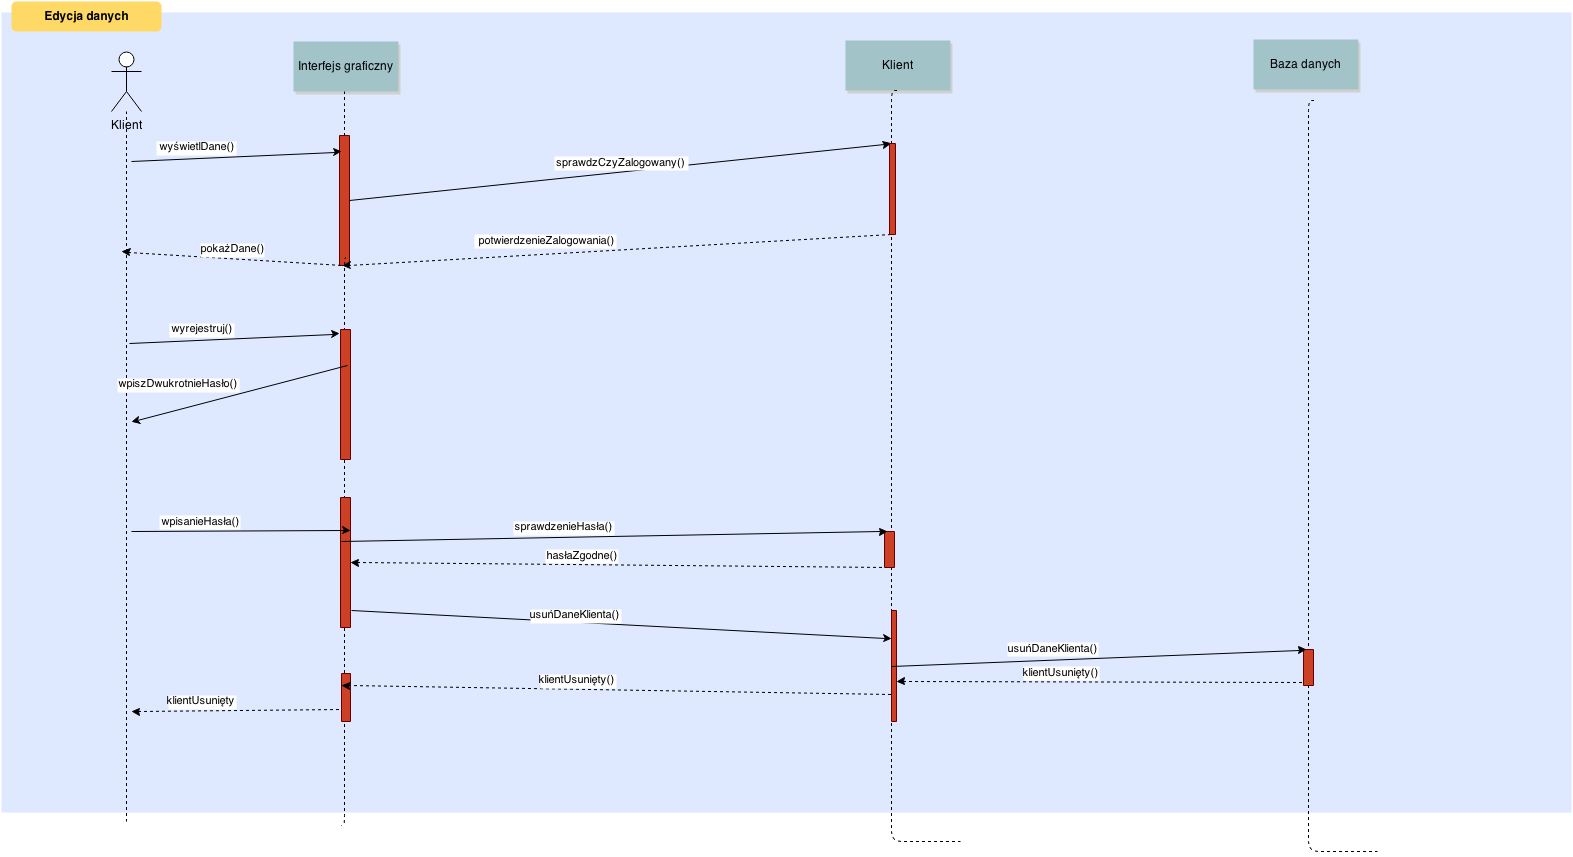
\includegraphics[width=\textwidth,
    height=0.5\textheight]{graphics/UseCase/Klient/WyrejestrowanieSieKlientaSD.png}
    \caption{Diagram sekwencji dla przypadku użycia Wyrejestrowanie Się Klienta
    - scenariusz główny}
\end{figure}
  
  
 